\chapter{Theoretical Background}

The construction of robust and efficient compilers relies heavily on a strong theoretical foundation. This chapter aims to establish the importance of these theoretical underpinnings by exploring the key areas that are fundamental to understanding and building the frontend of a compiler. 
These areas include the principles of formal languages, the distinct phases of the compilation process, the intricacies of lexical analysis, the methodologies of syntax analysis, and the design considerations for abstract syntax trees. 

A solid grasp of these theoretical concepts empowers compiler developers to make informed design decisions, effectively troubleshoot challenges, and ultimately create reliable and performant language processing tools. The ability to build a compiler from its foundational principles, as well as to leverage existing compiler construction tools and understand their inherent limitations, is significantly enhanced by a comprehensive theoretical understanding.

\section{Formal Languages}

\begin{definition}
\textbf{Formal language} is a precisely defined set of strings composed from a finite alphabet, with their structure and validity governed by a specific set of rules known as a formal grammar\cite{aho2007compilers}.
\end{definition}

Unlike natural languages, which evolve organically and often contain ambiguities, formal languages are intentionally designed for specific applications, such as mathematics, chemistry, and, most importantly for our context, programming. The notation employed by mathematicians to express relationships between numbers and symbols, for instance, constitutes a formal language adept at its intended purpose. Similarly, programming languages are formal languages meticulously crafted to express computations in an unambiguous manner \cite{runestone-formal-natural-languages}.

The fundamental building blocks of a formal language include a finite set of symbols known as the alphabet, from which finite sequences (strings or words) are constructed, and a subset of these strings that constitutes the language itself. The syntax of a formal language determines which strings are well‑formed according to a predefined set of production rules \cite{aho2007compilers, runestone-formal-natural-languages}. The design of a programming language necessitates a precise syntax to guarantee each program has a unique interpretation by the compiler.

\subsection{Types of Formal Languages}

Formal languages can be categorised into different types based on the complexity of their defining grammars, often visualised through the Chomsky hierarchy illustrated in Figure~\ref{figure:chomsky}. Within this hierarchy, regular languages and context‑free languages hold particular significance for compiler frontends \cite{aho2007compilers}.

\begin{figure}[ht]
\centering
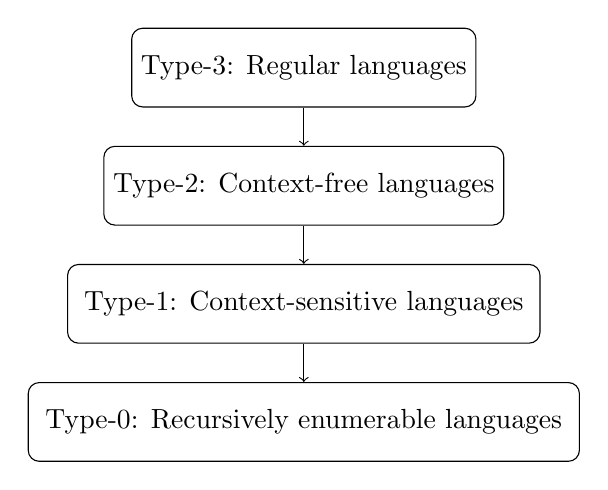
\begin{tikzpicture}[node distance=1.5cm]
\node (type3) [draw, rectangle, rounded corners=4pt, minimum width=4cm, minimum height=1cm] {Type‑3: Regular languages};
\node (type2) [draw, rectangle, rounded corners=4pt, minimum width=5cm, minimum height=1cm, below of=type3] {Type‑2: Context‑free languages};
\node (type1) [draw, rectangle, rounded corners=4pt, minimum width=6cm, minimum height=1cm, below of=type2] {Type‑1: Context‑sensitive languages};
\node (type0) [draw, rectangle, rounded corners=4pt, minimum width=7cm, minimum height=1cm, below of=type1] {Type‑0: Recursively enumerable languages};
\draw[->] (type3) -- (type2);
\draw[->] (type2) -- (type1);
\draw[->] (type1) -- (type0);
\end{tikzpicture}
\caption{Chomsky hierarchy of formal languages}
\label{figure:chomsky}
\end{figure}

\subsubsection*{Regular Languages}
Regular languages are the simplest in the hierarchy and can be defined using regular expressions, which offer a concise way to describe patterns of strings recognised by finite automata. In compilers, they are primarily used in lexical analysis to define tokens such as keywords, identifiers and operators \cite{aho2007compilers}.

\subsubsection*{Context‑Free Languages (CFLs)}
Context‑free languages, defined by context‑free grammars comprising production rules, are recognised by pushdown automata. The syntactic structure of programming languages—including hierarchical statements, expressions and control constructs—is typically defined using CFGs, and parsing relies on these principles \cite{kent-context-free-grammars-pda, aho2007compilers}.

While context‑sensitive and recursively enumerable languages appear in the Chomsky hierarchy, their direct relevance to compiler frontends is limited. Regular languages suffice for token recognition, whereas the intricate syntactic structures of programming languages demand the expressive power of context‑free languages.

\subsection{Key Properties of Formal Languages}

Understanding syntax, semantics and ambiguity is essential for comprehending how compilers process source code. Syntax governs token formation and program structure, semantics addresses the meaning and consistency checks during semantic analysis, and ambiguity—where a grammar permits multiple parse trees for the same string—is minimised in language design to ensure predictable compiler behaviour \cite{aho2007compilers}.

\subsection{The Significance of Formal Language Theory}

Formal language theory provides the mathematical tools and methodologies for specifying and implementing lexical analysers (via regular expressions and finite automata) and parsers (via context‑free grammars and parsing techniques). It guides the selection of appropriate formalisms, ensuring that compiler design proceeds systematically and reliably.

\pagebreak
